\documentclass[border=10pt]{standalone}
\usepackage{tikz}
\usetikzlibrary{shapes.geometric,shadows.blur}
\usepackage{amsmath}

\begin{document}

\centering
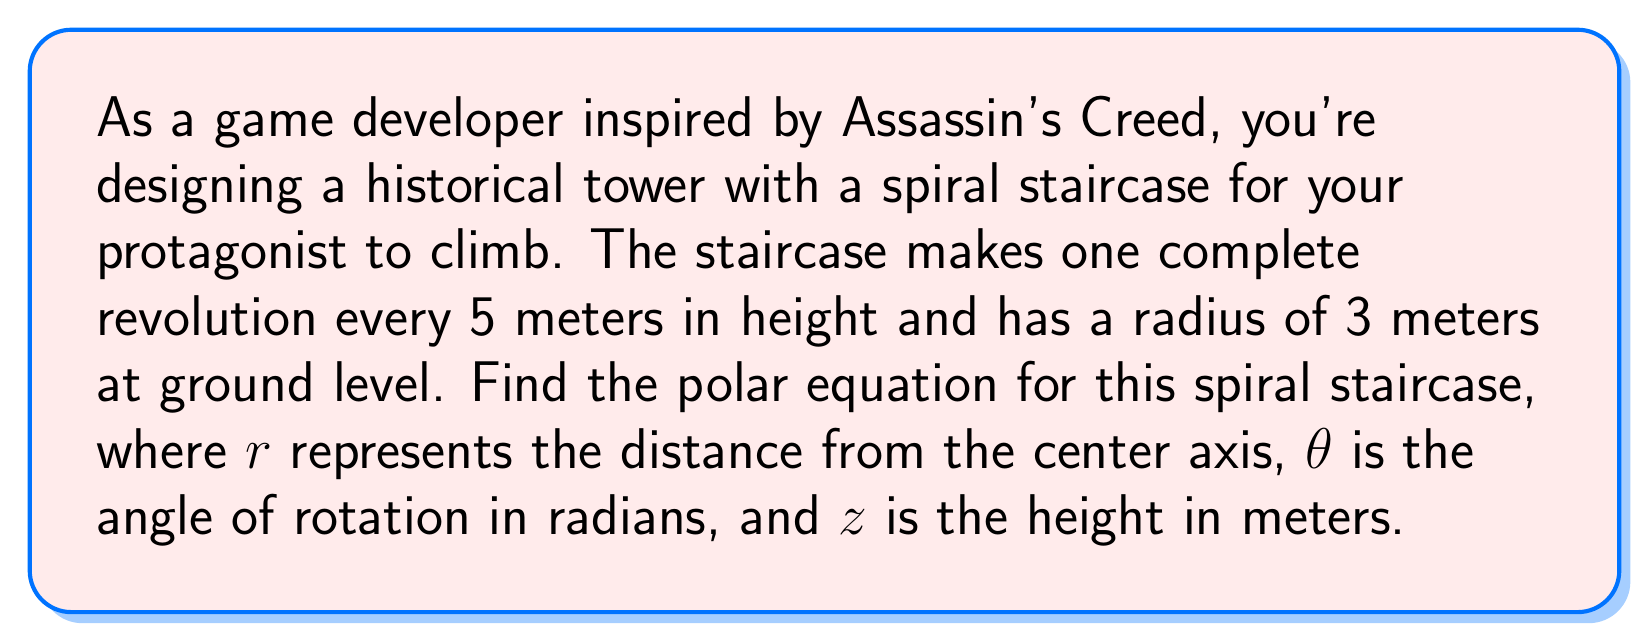
\begin{tikzpicture}
    \node[
        rectangle,
        rounded corners=15pt,
        draw=blue!55!cyan,
        line width=1.5pt,
        fill=red!8,
        drop shadow={shadow xshift=4pt, shadow yshift=-4pt, fill=blue!55!cyan, opacity=.35},
        text width=18.5cm,
        inner sep=24pt,
        align=flush left,
        font=\sffamily\fontsize{20}{24}\selectfont
    ] {
        As a game developer inspired by Assassin's Creed, you're designing a historical tower with a spiral staircase for your protagonist to climb. The staircase makes one complete revolution every 5 meters in height and has a radius of 3 meters at ground level. Find the polar equation for this spiral staircase, where $r$ represents the distance from the center axis, $\theta$ is the angle of rotation in radians, and $z$ is the height in meters.
    };
\end{tikzpicture}

\end{document}
